\documentclass[14pt]{beamer}
\usepackage[T2A]{fontenc}
\usepackage[utf8]{inputenc}
\usepackage[english]{babel}
\usepackage{amssymb,amsfonts,amsmath,mathtext}
\usepackage{cite,enumerate,float,indentfirst}
\usepackage{graphicx}
\usepackage{multicol}
\usepackage[boxed,algochapter,noline,czech]{algorithm2e}

\renewcommand{\vec}[1]{\ensuremath{\boldsymbol{#1}}}

\graphicspath{{images/}}

\usetheme{Pittsburgh}
\usecolortheme{whale}

\setbeamercolor{footline}{fg=blue}
\setbeamertemplate{footline}{
  \leavevmode%
  \hbox{%
  \begin{beamercolorbox}[wd=.333333\paperwidth,ht=2.25ex,dp=1ex,center]{}%
    Boris Kudryashov, ITMO University
  \end{beamercolorbox}%
  \begin{beamercolorbox}[wd=.333333\paperwidth,ht=2.25ex,dp=1ex,center]{}%
    St. Petersburg, 2016
  \end{beamercolorbox}%
  \begin{beamercolorbox}[wd=.333333\paperwidth,ht=2.25ex,dp=1ex,right]{}%
  Page \insertframenumber{} of \inserttotalframenumber \hspace*{2ex}
  \end{beamercolorbox}}%
  \vskip0pt%
}

\newcommand{\itemi}{\item[\checkmark]}

\title{\small{Information Theory. 3rd Chapter Slides}}
\author{\huge{
Boris Kudryashov \\
\vspace{30pt}
ITMO University
}}


\begin{document}

\maketitle

\begin{frame}
\frametitle{Agenda}
\begin{enumerate}    
% \footnotesize {
% \small{
    
\item Universal coding task
\item Useful combinatorial formulas
\item Two pass encoding
\item Enumerative coding
\item Asymptotic bounds of redundancy
\item Adaptive coding
\item Algorithm comparison

\end{enumerate}
\end{frame}

\begin{frame}
\frametitle{Universal coding task}
\begin{itemize}    
% \footnotesize {
% \small{
    
    \item  \textit{Encoding redundancy} for a model class $\Omega$ is
    \begin{equation}
    \label{redundancy}
     r_n(\Omega ) = \mathop {\sup }\limits_{ \omega \in \Omega }
    \left[ {\bar {R}_n(\omega)- H_\omega } \right].
    \end{equation}
    
    \item Coding is called \textit{Universal} if for algorithm holds
    \[
    \lim_{n\rightarrow \infty}  r_n(\Omega ) =0,
    \]
    
\end{itemize}
\end{frame}


% ----------------------Useful combinatorial formulas------------

\begin{frame}
\frametitle{Useful combinatorial formulas}
\begin{itemize}    
% \footnotesize {
% \small{
    
    \item Consider sequences $\vec x = (x_1 ,...,x_n )$, where $x_i$ has one of $M_i$ values, $i = 1,...,n$. Number of different $\vec x$ is
    \begin{equation}
    \label{eq3_1} \left| {\left\{ {\vec x = (x_1 ,...,x_n ):x_i \in
    \{0,...,M_i - 1\},i = 1,...n} \right\}} \right| = \prod\limits_{i = 1}^n {M_i } .
    \end{equation}
    
    \item 
    \begin{equation}
    \label{eq3_2}
    A_M^n = M(M - 1)\times ...\times (M - n + 1)
    =\frac{M!}{(M - n)!} .
    \end{equation}
    
\end{itemize}
\end{frame}


\begin{frame}
\frametitle{Useful combinatorial formulas}
\begin{itemize}    
% \footnotesize {
% \small{
    
    \item Number of combinations
    \begin{eqnarray}
    \label{eq3_4} C_M^n &=&\binom M n = \frac{A_M^n }{P_n }=\nonumber\\
    &=& \frac{M(M - 1)\times ...\times (M - n + 1)}{n!} =\nonumber\\
    &=& \frac{M!}{n!(M - n)!}.
    \end{eqnarray}
   
    \item Number of combinations
    \begin{equation}
    \label{eq3_5} %
    \binom n k = \left\{
    \begin{array} {cl}
    \frac {n!}{k!(n - k)!}, &\mbox{если } n\ge k\ge 0 \\
    1,       &\mbox{если } n\ge 0 \mbox{ и } k=0 \mbox{ или } k=n\\
    0,       &\mbox{если } k<0 \mbox{ или } k>n
    \end{array} \right 
    \end{equation}


\end{itemize}
\end{frame}


\begin{frame}
\frametitle{Useful combinatorial formulas}
\begin{itemize}    
% \footnotesize {
\small{

    \item binomial coefficient 
    \[
    (a + b)^n = \sum\limits_{k = 0}^n \binom n k  a^k b^{n-k}.
    \]
    
    \item Number os binary sequences of length $n$, which contain $\tau _1 $ ones and $\tau _0 = n - \tau _1 $ zeros.
    \begin{equation}
    \label{eq3_6} N(\tau _0 ,\tau _1 ) = \binom n {\tau _0}=
    \frac{n}{\tau _0 !\tau _1 !}.
    \end{equation}
    
    \item Composition of sequence $\vec x$ is vector $\vec \tau (\vec x) = (\tau _0 (\vec x),...,\tau _{M - 1} (\vec x))$, where $\tau _i (\vec x)$ denotes number of elements $x_t = i$ in sequence $\vec x = (x_1 ,...,x_n )$.
  
}
\end{itemize}
\end{frame}


\begin{frame}
\frametitle{Useful combinatorial formulas}
\begin{itemize}    
% \footnotesize {
\small{ 
    
    \item For $M=3$
    \[
    N(\vec \tau) = \binom  n {\tau _0 } \binom {n - \tau _0 } {\tau _1 } = \frac{n!}{\tau _0 !(n - \tau _0 )!}\frac{(n - \tau _0 )!}{\tau _1 !(n - \tau _0 - \tau _1 )!} = \frac{n!}{\tau _0 !\tau _1 !\tau _2 !}.
    \]
    
    \item For arbitrary $M$
    \begin{equation}
    \label{eq3_7} N(\vec \tau) = \frac{n!}{\tau _0 !...\tau _{M - 1} !}.
    \end{equation}
    
    \item Newton formula generalization
    \[
    (a_0 + ... + a_{M - 1} )^n = \sum\limits_{\vec \tau:~\tau _0 + ... + \tau _{M - 1} = n} {N(\vec \tau)\prod\limits_{i = 0}^{M - 1} {a_i^{\tau _i } } } .
    \]
}
\end{itemize}
\end{frame}


\begin{frame}
\frametitle{Useful combinatorial formulas}
\begin{itemize}    
% \footnotesize {
\small{
    
    \item Consider the following lemma:
    \begin{lemma} \label{num_comp} $n \in mathbb{N}$ can be written as sum of $M$ non-negative integer terms in $\binom  {n + M - 1} {M - 1} $ ways. 
    \end{lemma}

    \item Number of different compositions of sequence of length $n$ over $M$-size alphabet is
    \begin{equation}
    \label{eq3_8}
    N_\tau (n,M) = \binom {n + M - 1} {M - 1}
    \end{equation}
    
    \item Stirling formula
    \begin{equation}
    \label{eq3_9} \sqrt {2\pi n} n^ne^{ - n}\exp \left\{ {\frac{1}{12n + 1}} \right\} < n! < \sqrt {2\pi n} n^ne^{ - n}\exp \left\{ {\frac{1}{12n}} \right\}.
    \end{equation}  
 }   
\end{itemize}
\end{frame}


\begin{frame}
\frametitle{Useful combinatorial formulas}
\begin{itemize}    
% \footnotesize {
\small{    
    
    
    \item Consider
    \[
    N(\vec \tau) < (2\pi n)^{ - \frac{M - 1}{2}}2^{n\log n -
    \sum\limits_i {\tau _i \log \tau _i } }\left( {\prod\limits_i
    {\frac{n}{\tau _i }} } \right)^{1 / 2}\times
    \]
    \begin{equation}
    \label{eq3_10} \times \exp \left\{ {\frac{1}{12n} - \sum\limits_i
    {\frac{1}{12\tau _i + 1}} } \right\}.
    \end{equation}
    
    \item Logarithm of number of sequences with specified composition
    \begin{equation}
    \label{eq3_11} \log N(\vec \tau) < nH(\vec {\hat p}) - \frac{M -1}{2}\log (2\pi n) - \frac{1}{2}\sum\limits_i {\log (\hat {p}_i )} ,
    \end{equation}
}
\end{itemize}
\end{frame}


\begin{frame}
\frametitle{Useful combinatorial formulas}
\begin{itemize}    
% \footnotesize {
\small{
    
    \item More compact estimation
    \begin{equation}
    \label{eq3_12} \log N(\vec \tau) < nH(\vec {\hat p}) - \frac{M - 1}{2}\log (2\pi n) + \frac{1}{2}\log \frac{n}{n - M + 1}.
    \end{equation}
    
    \item Recurrent formula holds
    \begin{equation}
    \label{eq3_13} \binom {n+1} w =\binom n w+\binom n {w-1} .
    \end{equation}
    
    \item 
    \begin{equation}
    \label{eq3_14} \binom {n+1} w =\binom n w+ \binom {n-1} {w-1} + ... + \binom {n-w+1} 1.
    \end{equation}
} 
\end{itemize}
\end{frame}
    
% -----------------------Two pass encoding-------------


\begin{frame}
\frametitle{Two pass encoding}
\begin{itemize}    
\footnotesize {
% \small{

    \item 
    \begin{equation}
    \label{ex2pass} {\texttt{
    IF{\_}WE{\_}CANNOT{\_}DO{\_}AS{\_}WE{\_}WOULD{\_}WE{\_}SHOULD{\_}DO{\_}AS{\_}WE{\_}CAN} }\\
    \end{equation}
}
    \item 
    \[
    l_2 = 6 + 6 + 12\times 2 + 5\times 3 + ... + 6 = 178.
    \]
    
    \item 
    \begin{center}
    00010000010100110111101101111.
    \end{center}

\end{itemize}
\end{frame}
    

\begin{frame}
\frametitle{Two pass encoding}
\begin{itemize}    
% \footnotesize {
% \small{    
    
    \item 
    \[
    l_1 = 29 + 8\times 15 = 149\text{~bit}.
    \]
    
    \item 
    \begin{equation}
    \label{eq3_15} l = l_1 + l_2 = 149 + 178 = 327\text{~bit}.
    \end{equation}
   
\end{itemize}
\end{frame}

\begin{frame}
\frametitle{Two pass encoding}
\begin{itemize}    
% \footnotesize {
% \small{

    \begin{table}[htbp]
    \caption{Huffman code for text (\ref{ex2pass})}
    \begin{center}
    \scalebox{0.65}{
    \begin{tabular}{|c|c|c|l|}
    \hline %
    Character &Number of & Codeword& Codeword  \\
          &iterations &   length       &  \\\hline %
    I   & 1 & 6 & 010000 \\ \hline %
    F   & 1 & 6 & 010001 \\ \hline %
    {\_}& 12& 2&  00     \\ \hline %
    W   & 5 & 3 & 100    \\ \hline %
    E   & 4 & 4 & 0101   \\ \hline %
    C   & 2 & 5 & 01001  \\ \hline %
    A   & 4 & 4 & 1010   \\ \hline %
    N   & 3 & 4 & 1011   \\ \hline %
    O   & 5 & 3 & 110    \\ \hline %
    T   & 1 & 6 & 011110 \\ \hline %
    D   & 4 & 4 & 0110   \\ \hline %
    S   & 3 & 4 & 1110   \\ \hline %
    U   & 2 & 4 & 1111   \\ \hline %
    L   & 2 & 5 & 01110  \\ \hline %
    H   & 1 & 6 & 011111 \\\hline
    \end{tabular}
    }
    \end{center}
    \label{tab2pass}
    \end{table}
    
\end{itemize}
\end{frame}



\begin{frame}
\frametitle{Two pass encoding}
\begin{itemize}    
% \footnotesize {
% \small{

    \begin{figure}[ht]
    \begin{minipage}{1.0\linewidth}
    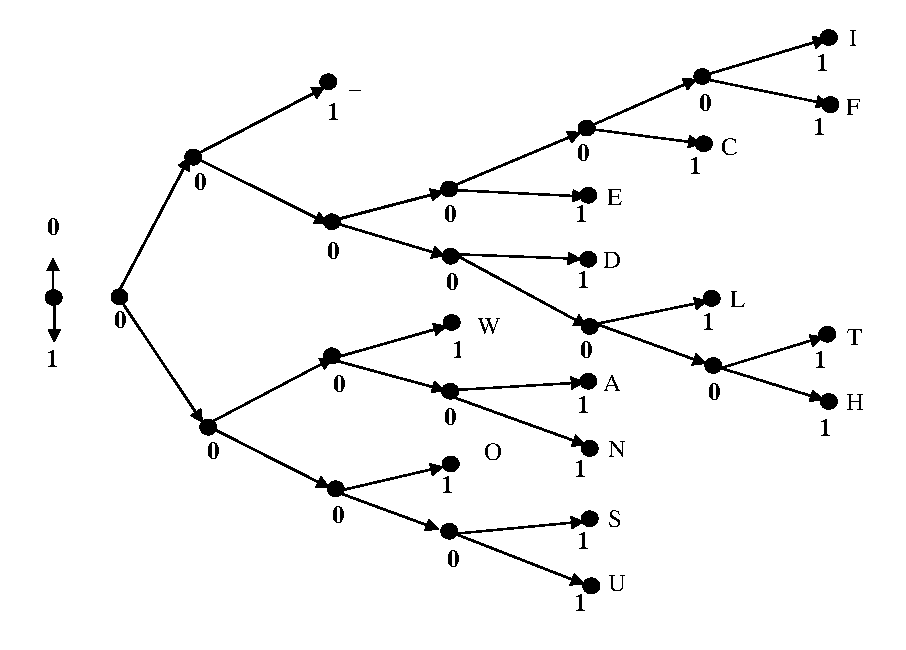
\includegraphics[width=1.0\textwidth]{fig3_1.eps}
    \caption{Huffman codetree for (\ref{ex2pass})}
    \label{HUF_tree}
    \end{minipage}
    \end{figure}
    
\end{itemize}
\end{frame}



\begin{frame}
\frametitle{Two pass encoding}
\begin{itemize}    
% \footnotesize {
% \small{
    \begin{table}[htbp]
    \label{tab2pass_reg} \caption{Regular Huffman code}
    \scalebox{0.65}{
    \begin{tabular}
    {|c|c|l|} \hline %
    Character & Codeword length & Codeword\\ \hline%
    {\_} & 2 & 00     \\ \hline %
    O    & 3 & 010    \\ \hline %
    W    & 3 & 011    \\ \hline %
    A    & 4 & 1000   \\ \hline %
    D    & 4 & 1001   \\ \hline %
    E    & 4 & 1010   \\ \hline %
    N    & 4 & 1011   \\ \hline %
    S    & 4 & 1100   \\ \hline %
    U    & 4 & 1101   \\ \hline %
    C    & 5 & 11100  \\ \hline %
    L    & 5 & 11101  \\ \hline %
    F    & 6 & 111100 \\ \hline %
    H    & 6 & 111101 \\ \hline %
    I    & 6 & 111110 \\ \hline %
    T    & 6 & 111111 \\ \hline
    \end{tabular}
    }
    \label{tab2}
    \end{table}
\end{itemize}
\end{frame}



\begin{frame}
\frametitle{Two pass encoding}
\begin{itemize}    
% \footnotesize {
% \small{

    \begin{table}[htbp]
    \caption{Number of bits for regular code tree transmitting}
    \scalebox{0.75}{
    \begin{tabular}
    {|c|c|c|c|c|}\hline %
    Level& Number of & Number of & Range of & Expenses  \\ %
        & nodes  &  leaves  $n_i $& values $n_i $&in bits \\ \hline %
    0& 1& 0& 0\ldots 1& 1 \\ \hline %
    1& 2& 0& 0\ldots 2& 2 \\ \hline %
    2& 4& 1& 0\ldots 4& 3 \\ \hline %
    3& 6& 2& 0\ldots 6& 3 \\ \hline %
    4& 8& 6& 0\ldots 8& 4 \\ \hline %
    5& 4& 2& 0\ldots 4& 3 \\ \hline %
    6& 4& 4& 0\ldots 4& 3 \\ \hline %
    Всего& \multicolumn{3}{c|}{}&19 \\ \hline %
    \end{tabular}
    }
    \label{tab_bits_for_tree}
    \end{table}
    
\end{itemize}
\end{frame}



\begin{frame}
\frametitle{Two pass encoding}
\begin{itemize}    
% \footnotesize {
% \small{
    \begin{figure}[ht]
    \begin{minipage}{1.0\linewidth}
    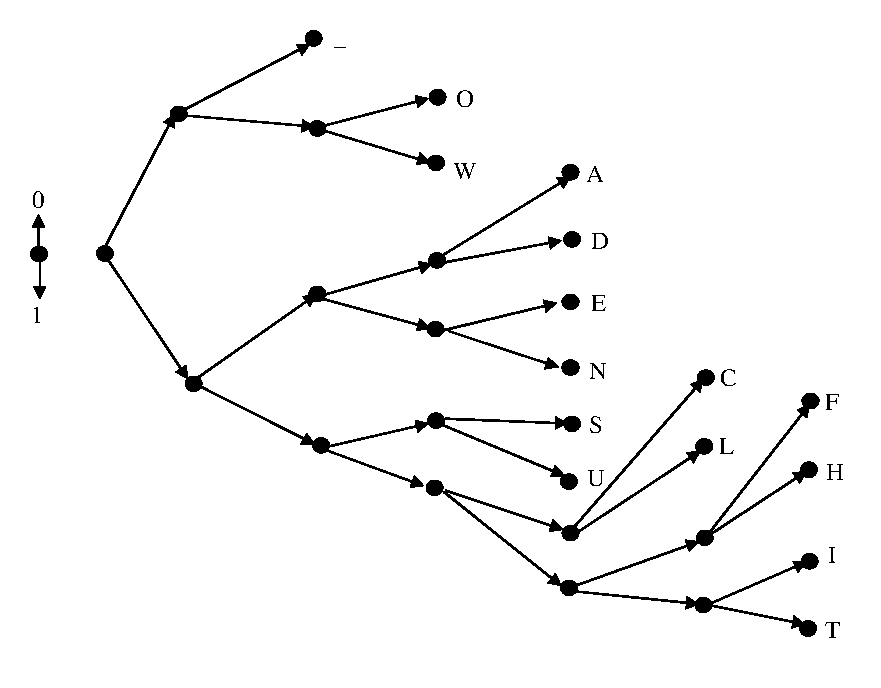
\includegraphics[width=1.0\textwidth]{fig3_2.eps}
    \caption{Codetree for regular Huffman code}
    \label{HUF_tree_reg}
    \end{minipage}
    \end{figure}
    
\end{itemize}
\end{frame}



\begin{frame}
\frametitle{Two pass encoding}
\begin{itemize}    
% \footnotesize {
% \small{

    \item Enough for transmitting information about letters that are associated with regular codetree nodes:
    \[
    \left\lceil \log \binom {256} 1 \right\rceil +%
    \left\lceil \log \binom {255} 2 \right\rceil +%
    \left\lceil \log \binom {253} 6 \right\rceil +%
    \]
    \[
    +
    \left\lceil \log \binom {247} 2 \right\rceil +%
    \left\lceil \log \binom {245} 4 \right\rceil =105 \text{~бит}
    \]
    
    \item More precise 
    \begin{equation}
    \label{eq3_16} l = 178 + 19 + 105 = 302\text{~бит} .
    \end{equation}
    
\end{itemize}
\end{frame}


\begin{frame}
\frametitle{Two pass encoding}
% \footnotesize {
% \small{

    \begin{theorem} \label{th_two_pass}
    For two pass coding with Huffman code of Discrete Memoryless Source with alphabet size $M$ and entropy $H$, average code rate satisfies
    \begin{equation}
    \label{eq3_17} \bar {R} \le H + 1 + \frac{1}{n}\left( {M\log M + 3M - 1} \right).
    \end{equation}
    \end{theorem}

\end{frame}



\begin{frame}
\frametitle{Two pass encoding}
Proof.
\begin{itemize}    

\small{

    \item
    \label{eq3_18} $l_1 (\vec x) \le 2M - 1 + M\left\lceil {\log M} \right\rceil \le M\log M + 3M - 1.$
}
\footnotesize {
    \item 
    \begin{eqnarray}
    \label{eq3_19}%
    l_2 (\vec x) &\stackrel{\rm (a)}{=}& \sum\limits_{i = 1}^n l(x_i )
    =\nonumber\\
    &\stackrel{\rm (b)}{=}& \sum\limits_{x \in X} \tau _n (x)l(x)=\nonumber\\
    &\stackrel{\rm (c)}{=}& n \sum\limits_{x \in X} \frac{\tau _n
    (x)}{n}l(x) =\nonumber\\
    &\stackrel{\rm (d)}{=}&  n\sum\limits_{x \in X} \hat {p}_n (x)l(x)= \nonumber\\
    &\stackrel{\rm (e)}{=}& n {\rm {\bf M}}_{\vec {\hat {p}}_n}\left[
    {l(x)} \right]\le \nonumber\\
    &\stackrel{\rm (f)}{\le}& n(H(\vec {\hat {p}}_n ) + 1).
    \end{eqnarray}
}

\end{itemize}
\end{frame}


\begin{frame}
\frametitle{Two pass encoding}
Proof.
\begin{itemize}    
% \footnotesize {
\small{

    \item
    \begin{eqnarray}
    \label{eq3_20}
    \bar {R}(\vec x) &=& \frac{l(\vec x)}{n} = \frac{l_1
    (\vec x) + l_2 (\vec x)}{n} \le \\
    &\le& H(\vec {\hat {p}}_n) + 1 + \frac{1}{n}\left( {M\log M + 3M -
    1} \right).
    \end{eqnarray}
    
    \item
    \begin{equation}
    \label{eq3_21} {\rm {\bf M}}\left[ {H(\vec {\hat {p}}_n} \right]
    \stackrel{\rm (a)}{\le} H\left( {{\rm {\bf M}}\left[\vec {\hat
    {p}}_n \right]} \right) \stackrel{\rm (b)}{=} H(\vec p)=H.
    \end{equation}
    
    
    \item
    \begin{equation}
    \label{eq3_22} {\rm {\bf M}}\left[ \vec {\hat {p}}_n \right] = \vec p,
    \end{equation}
    
    \item 
    \[
    {\rm {\bf M}}\left[ {\frac{\tau _n (a)}{n}} \right] = p(a),\mbox{ }a \in X.
    \]
}
\end{itemize}
\end{frame}


\begin{frame}
\frametitle{Two pass encoding}
Proof.
\begin{itemize}    
% \footnotesize {
\small{
       
    \item 
    \[
    \chi _a (x) = \left\{ {{\begin{array}{*{20}c}
     {1,\mbox{ при }x = a,} \hfill \\
     {0,\mbox{ при }x \ne a.} \hfill \\
    \end{array} }} \right.
    \]
    
    \item 
    \[
    {\rm {\bf M}}\left[ {\chi _a (x)} \right] = 1\times p(a) + 0\times
    (1 - p(a)) = p(a).
    \]
    
    \item 
    \begin{eqnarray*}
    {\rm {\bf M}}\left[ {\frac{\tau _n (a)}{n}} \right] &=&
    \frac{1}{n}{\rm {\bf M}}\left[ {\sum\limits_{i = 1}^n {\chi _a (x_i
    )} } \right] =\\
     &=& \frac{1}{n}\sum\limits_{i = 1}^n {{\rm {\bf M}}\left[ {\chi _a
    (x_i )} \right]} = \\
    &=& p(a),\mbox{ }a \in X.
    \end{eqnarray*}
}

\end{itemize}
\end{frame}


\begin{frame}
\frametitle{Two pass encoding}
\begin{itemize}    
% \footnotesize {
% \small{    
    
    \item Note, that coding redundancy satisfies
    \begin{equation}
    \label{eq3_23} r = \bar {R} - H \le 1 + \frac{K}{n},
    \end{equation}
    
    \item When using arithmetic coding, the redundancy can be achieved:
    \begin{equation}
    \label{eq3_24}
     r(n)=\frac{M-1}{n} \log n +\frac
    {K}{n},
    \end{equation}
    where $M$ alphabet size, $K$ is a constant.
    
\end{itemize}
\end{frame}


\begin{frame}
\frametitle{Two pass encoding}
\begin{itemize}    
% \footnotesize {
% \small{
    
\end{itemize}
\end{frame}




\begin{frame}
\frametitle{Algorithm comparison}
\begin{itemize}    
% \footnotesize {
% \small{
    
\footnotesize {
 
    \begin{table}[htbp]
    \caption{Universal coding algorithm comparison}
    \begin{center}
    \begin{tabular}
    {|c|c|c|c|}  \hline %
    Algorithm & Number of  & Asymptotic &   codeword length  \\ %
              & traverses  & redundancy &   for text (\ref{ex2pass})    \\%
    \hline %
    2-traverse  & 2& $1 + K_1 / n$& 302 \\%
    coding, &  &  &  \\ %
    Huffman code &  &  &  \\ \hline%
    Enumerative & 2& $\frac{M\log n + K_3 }{2n}$& 283 \\ %
    coding      &  &  &  \\\hline %
     Adaptive & 1& $\frac{M\log n + K_4 }{2n}$& 291 \\%
     coding (A) &  &  &   \\\hline %
    Adaptive  & 1& $\frac{M\log n + K_5 }{2n}$&283 \\%
    coding (D) &  &  &  \\\hline
    \end{tabular}
    \label{tab3_6} \end{center}
    \end{table}
}    
    
\end{itemize}
\end{frame}

% \item Universal coding task
% \item Useful combinatorial formulas
% \item Two pass encoding
% \item Enumerative coding
% \item Asymptotic bounds of redundancy
% \item Adaptive coding
% \item Algorithm comparison


\end{document}